    %%%%%%%%%%%%%%%%%%%%%%%%%%%%%%%%%%%%%%%%%%%%%%%%%%%%%%%%%%%%
%%  This Beamer template was created by Cameron Bracken.
%%  Anyone can freely use or modify it for any purpose
%%  without attribution.
%%
%%  Last Modified: January 9, 2009
%%

\documentclass[xcolor=x11names,compress]{beamer}

%% General document %%%%%%%%%%%%%%%%%%%%%%%%%%%%%%%%%%
	\usepackage{graphicx}
	\usepackage{pgfplots}
	\usepackage{listings}
	\usepackage{tikz}
	\usepackage{siunitx}
	\usepackage{tikz}
	\usetikzlibrary{arrows,automata}
	\usepackage{siunitx}
	\usepackage{pgf}
	\usetikzlibrary{arrows}
	\usetikzlibrary{decorations.fractals, arrows}
	\usetikzlibrary{arrows,decorations.pathreplacing}
	\usepackage{xcolor}
	\usetikzlibrary{arrows, shapes, calc}
%%%%%%%%%%%%%%%%%%%%%%%%%%%%%%%%%%%%%%%%%%%%%%%%%%%%%%

%% Beamer Layout %%%%%%%%%%%%%%%%%%%%%%%%%%%%%%%%%%
	\useoutertheme[subsection=false,shadow]{miniframes}
	\useinnertheme{default}
	\usefonttheme{serif}
	\usepackage{palatino}
	\setcounter{tocdepth}{1}

	\setbeamerfont{title like}{shape=\scshape}
	\setbeamerfont{frametitle}{shape=\scshape}

	\setbeamercolor*{lower separation line head}{bg=DeepSkyBlue4}
	\setbeamercolor*{normal text}{fg=black,bg=white}
	\setbeamercolor*{alerted text}{fg=red}
	\setbeamercolor*{example text}{fg=black}
	\setbeamercolor*{structure}{fg=black}

	\setbeamercolor*{palette tertiary}{fg=black,bg=black!10}
	\setbeamercolor*{palette quaternary}{fg=black,bg=black!10}

% Page numbering
	\addtobeamertemplate{navigation symbols}{}{%
	    \usebeamerfont{footline}%
	    \usebeamercolor[fg]{footline}%
	    \hspace{1em}%
	    \insertframenumber/\inserttotalframenumber
	}

	\renewcommand{\(}{\begin{columns}}
	\renewcommand{\)}{\end{columns}}
	\newcommand{\<}[1]{\begin{column}{#1}}
	\renewcommand{\>}{\end{column}}
	\tikzset{onslide/.code args={<#1>#2}{%
	  \only<#1>{\pgfkeysalso{#2}} % \pgfkeysalso doesn't change the path
	}}  
%%%%%%%%%%%%%%%%%%%%%%%%%%%%%%%%%%%%%%%%%%%%%%%%%%

% Remove navigation
	\beamertemplatenavigationsymbolsempty
%%%%%%%%%%%%%%%%%%%%%%%%%%%%%%%%%%%%%%%%%%%%%%%
\begin{document}
	
\begin{frame}
\title{\huge Predicting LoL using Machine Learning on Big Data}
%\subtitle{SUBTITLE}

\author{
	Mathias Meldgaard Andersen\\
	Kent Munthe Caspersen\\
	Andreas Berre Eriksen\\
	Sander Jespersen\\
	Mikkel Alexander Madsen\\
	Anders Roland Nielsen\\
}

\titlepage
\end{frame}

\begin{frame}{Table of Contents}
\tableofcontents
\end{frame}

\section{\scshape Introduction}
\subsection{Motivation}

\begin{frame}{Motivation}
\begin{itemize}
\item item1
\begin{itemize}
\item item2
\end{itemize}
\end{itemize}
\vspace{20cm}
\end{frame}

\begin{frame}{Motivation}
\begin{itemize}
\item item1
\begin{itemize}
\item item2
\item item3
\end{itemize}
\end{itemize}
\vspace{20cm}
\end{frame}

	\begin{frame}{Game setup and data extraction}
\begin{itemize}
\item Basic 5x5 game setup
\begin{itemize}
\item A game consists of 10 summoners, 5 on each team, each summoner selects a champion to play on a lane, the summon also selects which summoners spellsm runes and masteries the summoner want to help boost the champion selected.   
\item Lanes: \{top, middel, jungle, bottom\}
\item Summoner(player): \{level ,champion, summoner spells, runes, masteries\}
\item Champion: \{level, passive, 3 tallents, 1 ulti, items\}
\end{itemize}
\end{itemize}
\vspace{20cm}
\end{frame}
\begin{frame}{Champion example}
\begin{figure}[h!]
\centering
\includegraphics[width=4cm]{leagueoflegends/ashe1}
\includegraphics[width=4cm]{leagueoflegends/ashe2}
\includegraphics[width=4cm]{leagueoflegends/volly}
\caption{Ashe's stats, spells and example}
\end{figure}
\end{frame}
\begin{frame}{Match objectives}
\begin{itemize}
\item Nesus, one for each team 
\item Inhibitor 3 for each team 
\item Tower 11 for each team 
\item Baron 1 in total
\item Dragon 1 in total
\item Gold and experience
\item Killing enermies, minions and monsters 
\end{itemize}
\end{frame}
\begin{frame}{Map}
\begin{figure}[h!]
\centering
\includegraphics[width=\linewidth, height=\textheight]{leagueoflegends/map}
\caption{Map of a classical 5x5 match}
\end{figure}
\end{frame}
	\begin{frame}{Features}
\centering
\includegraphics[scale=0.2]{img/kent/lolmap.jpg}
\end{frame}

\begin{frame}{Features}
\centering
\includegraphics[scale=0.35]{img/kent/1.png}\\
\vspace{8pt}
$P(Winner = \textcolor{blue}{\text{blue}}) = \alpha$
\end{frame}

\begin{frame}{Features}
\centering
\includegraphics[scale=0.35]{img/kent/2.png}\\
\vspace{8pt}
$P(Winner = \textcolor{purple}{\text{purple}}) = \alpha ?$
\end{frame}

\begin{frame}{Features}
\centering
\textcolor{blue}{Team blue} (won)
\includegraphics[scale=0.4]{img/kent/pickblue.png}\\
\vspace{20pt}
\textcolor{purple}{Team purple} (lost)
\includegraphics[scale=0.4]{img/kent/pickpurple.png}\\
\end{frame}

\begin{frame}{Binary representation}
\centering
\textcolor{blue}{Team blue} (won) \hspace{40pt} \textcolor{purple}{Team purple} (lost)\\
\includegraphics[width=0.47\textwidth]{img/kent/pickblue.png}\hspace{2pt}%
\includegraphics[width=0.47\textwidth]{img/kent/pickpurple.png}\\
\vspace{18pt}
$x =$\\
\hspace{2pt} $(\textcolor{blue}{0,\;1,\;0,\;0,\;1,\;1,\;0,\;1,\;1,\;0,\;...},\textcolor{purple}{1,\;0,\;1,\;1,\;1,\;0,\;0,\;0,\;1,\;0,...})$\\
\vspace{18pt}
$y = \textcolor{blue}{\text{true}}$
\end{frame}

\begin{frame}{Mirrored binary representation}
\centering
\textcolor{blue}{Team blue} (won) \hspace{40pt} \textcolor{purple}{Team purple} (lost)\\
\includegraphics[width=0.47\textwidth]{img/kent/pickblue.png}\hspace{2pt}%
\includegraphics[width=0.47\textwidth]{img/kent/pickpurple.png}\\
\vspace{18pt}
$x =$\\
\hspace{2pt} $(\textcolor{blue}{0,\;1,\;0,\;0,\;1,\;1,\;0,\;1,\;1,\;0,\;...},\textcolor{purple}{1,\;0,\;1,\;1,\;1,\;0,\;0,\;0,\;1,\;0,...})$\\
$y = \textcolor{blue}{\text{true}}$\\
\vspace{18pt}
$x' =$\\
\hspace{2pt} $(\textcolor{purple}{1,\;0,\;1,\;1,\;1,\;0,\;0,\;0,\;1,\;0,...},\textcolor{blue}{0,\;1,\;0,\;0,\;1,\;1,\;0,\;1,\;1,\;0,\;...})$\\
$y' = \textcolor{purple}{\text{false}}$
\end{frame}

\begin{frame}{Compact binary representation}
\centering
\textcolor{blue}{Team blue} (won):\\
\hspace{20pt}\includegraphics[width=0.47\textwidth]{img/kent/pickblue.png}\\
\vspace{8pt}
$x = (\textcolor{blue}{0,\;1,\;0,\;0,\;1,\;1,\;0,\;1,\;1,\;0,\;...})$\\
$y = \textcolor{blue}{\text{true}}$\\
\vspace{40pt}
\textcolor{purple}{Team purple} (lost):\\
\hspace{20pt}\includegraphics[width=0.47\textwidth]{img/kent/pickpurple.png}\\
\vspace{8pt}
$x' = (\textcolor{purple}{1,\;0,\;1,\;1,\;1,\;0,\;0,\;0,\;1,\;0,\;...})$\\
$y' = \textcolor{purple}{\text{false}}$
\end{frame}

\begin{frame}{Ternary representation}
\centering
\textcolor{blue}{Team blue} (won)\\
\hspace{20pt}\includegraphics[scale=0.31]{img/kent/pickblue.png}\\
\vspace{20pt}
\textcolor{purple}{Team purple} (lost)\\
\hspace{20pt}\includegraphics[scale=0.31]{img/kent/pickpurple.png}\\
\vspace{20pt}
$x = (\textcolor{purple}{-1},\;\textcolor{blue}{1},\,\textcolor{purple}{-1},\textcolor{purple}{-1},\;0,\;\,\textcolor{blue}{1},\;\;0,\;\,\,\textcolor{blue}{1},\;\;0,\;\;0,\;\,...)$\\
$y = \textcolor{blue}{\text{true}}$\\
\end{frame}

\begin{frame}{Features}
\centering
\begin{figure}[!htb]
  \centering
  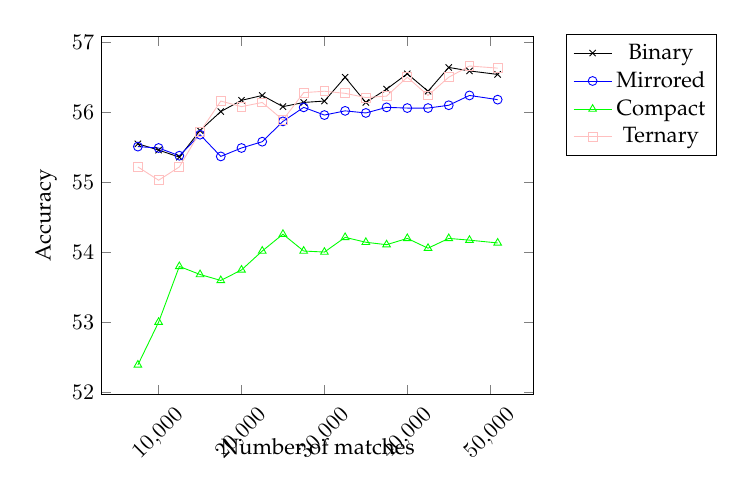
\begin{tikzpicture}[scale=0.8] 
    \begin{axis}[
      xlabel=Number of matches, 
      ylabel=Accuracy,
      xtick={10000,20000,30000,40000,50000},
      xticklabel style={rotate=45,anchor=near xticklabel},
      scaled x ticks=false,
      x label style={at={(axis description cs:0.5,-0.1)},anchor=north},
      legend style={at={(1.25,1.005)},
        anchor=north,legend columns=1},] 
      \addplot[color=black,mark=x] coordinates { 
        (7500, 55.55)
        (10000, 55.46)
        (12500, 55.36)
        (15000, 55.74)
        (17500, 56.01)
        (20000, 56.17)
        (22500, 56.24)
        (25000, 56.08)
        (27500, 56.14)
        (30000, 56.16)
        (32500, 56.50)
        (35000, 56.14)
        (37500, 56.33)
        (40000, 56.55)
        (42500, 56.30)
        (45000, 56.64)
        (47500, 56.59)
        (50901, 56.54)
      };
      \addplot[color=blue,mark=o] coordinates { 
        (7500, 55.51)  
        (10000, 55.49)
        (12500, 55.38)
        (15000, 55.68)
        (17500, 55.37)
        (20000, 55.49)
        (22500, 55.58)
        (25000, 55.87)
        (27500, 56.07)
        (30000, 55.96)
        (32500, 56.02)
        (35000, 55.99)
        (37500, 56.07)
        (40000, 56.06)
        (42500, 56.06)
        (45000, 56.10)
        (47500, 56.24)
        (50901, 56.18)
      };
      \addplot[color=green,mark=triangle] coordinates { 
        (7500, 52.395)  
        (10000, 53.005)
        (12500, 53.80)
        (15000, 53.685)
        (17500, 53.60)
        (20000, 53.75)
        (22500, 54.02)
        (25000, 54.26)
        (27500, 54.02)
        (30000, 54.005)
        (32500, 54.215)
        (35000, 54.145)
        (37500, 54.11)
        (40000, 54.20)
        (42500, 54.06)
        (45000, 54.20)
        (47500, 54.175)
        (50901, 54.135)
      };
      \addplot[color=pink,mark=square] coordinates {
        (7500, 55.22)  
        (10000, 55.03)
        (12500, 55.22)
        (15000, 55.72)
        (17500, 56.16)
        (20000, 56.08)
        (22500, 56.14)
        (25000, 55.89)
        (27500, 56.28)
        (30000, 56.30)
        (32500, 56.27)
        (35000, 56.21)
        (37500, 56.23)        
        (40000, 56.50)
        (42500, 56.24)
        (45000, 56.50)
        (47500, 56.66)
        (50901, 56.63)
      };
      \legend{Binary, Mirrored, Compact, Ternary}
    \end{axis} 
  \end{tikzpicture}
\end{figure}
\end{frame}

\begin{frame}{Features}
\centering
10 different types of features:\\
\begin{itemize}
\item Single champions
\item Pairs of champions
\item Champion counters
\item Player ranks (captured in 3 different ways)
\item Champion lanes
\item Champion spells
\item Champion runes
\item Champion masteries
\end{itemize}
\end{frame}


\begin{frame}{Features}
\centering
FeatureCreator:
\begin{itemize}
\item Introducing new features
\item Combining features
\end{itemize}
\end{frame}

\begin{frame}{Features}
Introducing a new type of feature:
\begin{itemize}
\item Initialiser function: Provide the name of all possible features
\item Feature extractor function: Given a game object, identify the features present in that game
\end{itemize}
\end{frame}

\begin{frame}{Features}
Introducing feature $\phi_\text{SINGLE}$
\begin{itemize}
\item Initialiser function: 
	\begin{itemize}
	\item $\text{BLUE-Ahri}$
	\item $\text{BLUE-Akali}$
	\item ...
	\item $\text{BLUE-Zyra}$
	\item $\text{PURPLE-Akali}$
	\item $\text{PURPLE-Ahri}$
	\item ...
	\item $\text{PURPLE-Zyra}$
	\end{itemize}
\item Feature extractor function:  
	\begin{itemize}
	\item Game object $\rightarrow \{\text{BLUE-Olaf}, \text{BLUE-Ryze}, \text{PURPLE-Lulu}, ...\}$
	\end{itemize}
\end{itemize}
\end{frame}

\begin{frame}{Features}
Introducing feature $\phi_\text{SINGLE-CHAMPION}$
\begin{itemize}
\item Initialiser function:
	\begin{itemize}
	\item $\text{BLUE-Ahri} \rightarrow 1$
	\item $\text{BLUE-Akali} \rightarrow 2$
	\item ...
	\item $\text{BLUE-Zyra} \rightarrow m+124$
	\item $\text{PURPLE-Akali} \rightarrow m+125$
	\item $\text{PURPLE-Ahri} \rightarrow m+126$
	\item ...
	\item $\text{PURPLE-Zyra}\rightarrow m+248$
	\end{itemize}
\item Feature extractor function:  
	\begin{itemize}
	\item Game object $\rightarrow \{87, 96, 168, ...\}$
	\end{itemize}
\end{itemize}
\end{frame}	
	\begin{frame}{title}
\begin{itemize}
\item item1
\begin{itemize}
\item item2
\end{itemize}
\end{itemize}
\vspace{20cm}
\end{frame}
	\input{bigdataandcluster/bigdataandcluster.tex}
	\section{Experiments}
\subsection{Results}
\begin{frame}{Accuracy convergance}
\begin{minipage}{0.55\linewidth} 
%\begin{tikzpicture}[scale=0.70]
%  \begin{axis}[
%    ybar,
%    ylabel = Accuracy,
%    xlabel = Training size,
%    tick label style={font=\small},
%    tickpos=left,
%    xticklabels={6\%, 12\%, 25\%, 50\%, 100\%}, 
%    xtick={1,2,3,4,5, 6},
%    ymin=56,
%    legend entries={Training,Test},
%    legend style={at={(0.165,1.25)}, anchor=north,legend columns=1},
%    legend image code/.\cite{} ode={\draw[#1] (0cm,-0.1cm) rectangle (0.6cm,0.1cm);},   
%    ]   
%    \addplot +[bar shift=-.2cm] coordinates {(1,60.49) (2,59.66) (3,59.06) (4,58.85) (5,58.73)  };
%    \addplot +[bar shift=.2cm]coordinates {(1,58.28) (2,58.36) (3,58.38) (4, 58.46) (5,58.50) };
%  \end{axis}
%\end{tikzpicture}
\end{minipage}
\begin{minipage}{0.40\linewidth} 
\begin{itemize}
\item All prematch features
\item Logistic regression
\item Stochastic gradient descent 
\item L2-regularisation (regularisation factor of 0.01)
\end{itemize}
\vspace{0.05cm}
\begin{itemize}
\item Increased test data size gives no visible benefit
\item Increased training data size lowers overfitting
\end{itemize}
\end{minipage}
\end{frame}

\begin{frame}{Feature experiments}
\begin{minipage}{0.55\linewidth} 
%\begin{tikzpicture}[scale=0.70]
%\begin{axis}[
%ybar,
%ylabel = Accuracy,
%xlabel = Feature set,
%tick label style={font=\small},
%tickpos=left,
%xticklabels={1, 2, 3, 4, 5, 6}, 
%xtick={1,2,3,4,5, 6},
%ymin=53,
%legend entries={Training,Test},
%legend style={at={(0.165,1.25)}, anchor=north,legend columns=1},
%legend image code/.code={\draw[#1] (0cm,-0.1cm) rectangle (0.6cm,0.1cm);},   
%]   
%\addplot +[bar shift=-.2cm] coordinates {(1,55.12) (2,55.34) (3,55.31)  (4,55.58)     (5,56.08) (6, 58.73)};

%\addplot +[bar shift=.2cm]coordinates {(1,55.01) (2,54.98) (3,55.22) (4,  55.46) (5,55.92) (6, 58.50)};

%\end{axis}
%\end{tikzpicture}
\end{minipage}    
\begin{minipage}{0.40\linewidth}
\footnotesize{
\begin{enumerate}
\item $\phi_\text{SINGLE}$
\item $\phi_\text{PAIR}$
\item $\phi_\text{SINGLE}$, $\phi_\text{PAIR}$
\item $\phi_\text{SINGLE}$, $\phi_\text{PAIR}$, $\phi_\text{COUNTER}$
\item $\phi_\text{SINGLE}$, $\phi_\text{PAIR}$, $\phi_\text{COUNTER}$, $\phi_\text{BEST-RANK}$
\item $\phi_\text{SINGLE}$, $\phi_\text{PAIR}$, $\phi_\text{COUNTER}$, $\phi_\text{BEST-RANK}$, $\phi_\text{PLAYER-RANK}$, $\phi_\text{LANE-RANKS}$, $\phi_\text{LANE-CHAMPION}$, $\phi_\text{CHAMPION-SPELLS}$, $\phi_\text{CHAMPION-RUNES}$, $\phi_\text{CHAMPION-MASTERIES}$
\end{enumerate}
}
\end{minipage}
\end{frame}


\subsection{Knowledge extraction}
\begin{frame}{Accuracy}
\begin{itemize}
\item Reasons for low accuracy:
\begin{itemize}
\item Features not thoroughly  representative
\item Highest accuracy achieved
\end{itemize}
\item Combination of features:
\begin{itemize}
\item Accuracy not better when rank based features are combined
\item Different features does cause better accuracy
\end{itemize}
\end{itemize}
\end{frame}

\begin{frame}{Notable weights}
  \begin{itemize}
  \item No weights that standout by a lot
  \item Mostly symmetric around 0
  \end{itemize}
  \vspace{0.05cm}
  \begin{itemize}
  \item Negative for Blue:
    \begin{itemize}
    \item Jinx-BLUE-VS-LeeSin-PURPLE
    \item Blitzcrank-BLUE-VS-LeeSin-PURPLE
    \end{itemize}
  \item Positive for Blue:
    \begin{itemize}
    \item LeeSin-BLUE-VS-Blitzcrank-PURPLE
    \end{itemize}
  \item Possible reason:
    \begin{itemize}
    \item Blitzcrank can pull enemies in
    \item LeeSin can jump away
    \end{itemize}
  \end{itemize}
\end{frame}

\subsection{Conclusion}
\label{sec-1-3}
\begin{frame}[label=sec-1-3-1]{Conclusion}
\begin{itemize}
\item Worked with large dataset of 456GB
\item Cluster of 4 machines, 3 workers and 1 master running HDFS and Apache spark
\item Best accuracy achieved is 58.5\% using logistic regression
\begin{itemize}
\item Most likely as a consequence of balanced game
\end{itemize}
\item Results can be used for a tool that helps LoL players pick a winning champion or team
\end{itemize}
\end{frame}
\begin{frame}[label=sec-1-3-2]{Future work}
\begin{itemize}
\item Add additional features
\item If size of cluster is increased, better fault tolerance could be added
\item Evaluation of a game while it is going on
\begin{itemize}
\item This would increase the number of features by a lot
\item Based on events happening in the game, e.g. the dragon getting killed
\end{itemize}
\item An agent that could play optimally
\end{itemize}
\end{frame}
\end{document}
